\documentclass[12pt,preprint]{aastex}

\begin{document}
\def\simlt{\lower.5ex\hbox{$\; \buildrel < \over \sim \;$}}
\def\simgt{\lower.5ex\hbox{$\; \buildrel > \over \sim \;$}}

\title {LAB 1 -- \today \\ EXPLORING DIGITAL SAMPLING, FOURIER TRANSFORMS, and
  both DSB and SSB MIXERS}

\tableofcontents

	The purpose of this lab is to experimentally investigate digital
sampling, digital Fourier transforms, and mixers. Mixers are the basis
of heterodyne spectroscopy. Heterodyne spectroscopy, in turn, is what
you use every day that you listen to a radio, use a cell phone, watch
TV---or do radio astronomy. In the second lab, we'll use it
to observe the 21-cm line emission from our Galaxy.

In this lab, you will be performing several experiments, analyzing the
data and generating a number of different data files. You will need to
keep careful notes in your {\bf lab notebook}! Or, pay the penalty, and
forget what you did, do things twice, and be completely
disorganized. Your choice!

\section{GOALS} \label{goals}

\begin{itemize}

\item Learn how to sample electronic signals---here, one or more sine
  waves---digitally using our computers.

\item Get started with our programming language, Python, using it for the
  mathematical analysis, signal processing, and making nice plots.

\item Become acquainted with aliasing and the basic law of sampling: the
  Nyquist criterion.

\item Learn how to use Digital Fourier Transforms (or Discrete Fourier
  Transforms; DFT) to determine the frequency power spectrum of a time
  series. Understand leakage power and frequency resolution when
  sampling a single sine wave.

\item Learn about the Fast Fourier Transform (FFT) as a fast
  implementation of the DFT.

\item Learn how the FT treats noise, which is the important case for
  radio astronomy.

\item Learn about correlation functions and, in particular,
  autocorrelation functions and power spectra.

\item Learn the basics of mixing for frequency conversion (that's
  the {\it heterodyne} technique). Explore how real mixers differ from
  the ideal.

\item Learn how complex inputs to a FT break the negative/positive
  frequency degeneracy.

\item Construct a sideband-separating (SSB) mixer and explore the mixing
  process.
  

\item Learn enough Latex to write up your results in a formal lab
  report, including nice plots and graphs.

\end{itemize}

\section{SCHEDULE}

There's a lot to do in this lab! If you don't understand the Nyquist criterion
by the end of the first week, you're behind. Here's how it should be:
\begin{enumerate}

\item {\it The First Week. For class on 23 Jan:} Finish \S
  \ref{nyquist}, which requires reading the accompanying
  material in \S \ref{pwrspectrum}. {\it Be prepared to show your work, your
  software, and your results to the class, making real-time plots in
  Python during your presentation.}

\item {\it The Second Week. For class on 30 Jan:} Finish \S
  \ref{mixersect} and the reading in \S \ref{hetereo}. Again, be prepared
  to strut your stuff to the class.

\item {\it The Third Week. For class on 6 Feb:} Read the handouts in \S
  \ref{report}, and then write and hand in your formal report!  Your
  report should contain relevant plots together with commentary to
  illustrate your work, your thought processes, and your conclusions.
  Generally speaking, your lab report should address, with discussion
  and/or plots, each of the goals in \S \ref{goals}.

\end{enumerate}

\section{IN THE LAB: DIGITALLY SAMPLING A SINGLE SINE WAVE (First
  Week)}
\label{nyquist}
%
\subsection{Handouts and Software}
As you begin real work this first week, you will need to become immersed
in the Linux operating system, the Emacs editor, and Python. To this end,
you'll need to become familiar with the following handouts and Python
procedures:

\subsubsection{Handouts}
\begin{enumerate}
\item Learning Linux: {\tt unixprimer.pdf} ``A SHORT UNIX PRIMER'' Basic
  commands for Linux/Unix operating systems. Eventually you'll want to
  know all of the commands in here because they are so useful.

\item Learning the EMACS editor: {\tt emacs-beg.pdf} {\it ``A Beginners
  Guide to Emacs''} and the related {\tt emacskeyops.pdf} ``Common
  Editing Tasks and Their EMACS Keystroke Counterparts''. Emacs is
  excellent for everything, including editing writing computer
  code. Efficient editing means using the keyboard instead of the mouse;
  the second handout gives keystroke commands for the most commonly
  needed editing sequences.

\item Getting into Python: {\tt idltut1\_ay121.pdf} {\it ``Quick Python
  Tutorial Number One for AY121''} Gives you the basics of Python.

\item Plotting in Python: {\tt bpidl.pdf} {\it ``BPPython---BASIC PLOTTING IN
  Python: PLOTS, MULTIPLE PLOTS, COLORS, MAKING POSTSCRIPT FILES''} Sections
  1 and 2 are enough for now.

\item {\it This handout is optional}, because for this lab you can get
  along with just the material below in \S \ref{pwrspectrum}. This handout
  is more detailed, 28 pages of all you need to know about Discrete
  Fourier transforms.  {\tt fourierc.pdf} {\it ``DISCREETLY FINE TIMES
    with DISCRETE FOURIER TRANSFORMS (DFT’s with DFT’s) or “WHY DOES
    THAT FFT OUTPUT LOOK SO sWEIRD???” ''}.
\end{enumerate}
%
\subsubsection{Python Procedures}
The  following Python procedures are needed or useful for this
lab: \begin{enumerate}

\item {\tt getpico.pro} --- runs the A/D board to digitally sample
  signals. This is essential.

%\item {\tt srs1\_frq.pro} --- sets the frequency of one of the SRS
%  function generators. If you are lazy, you can set the SRSs by hand. If
%  you are creatively lazy, you will want to use {\tt srs1\_frq.pro}.

%\item {\tt srs1\_dbm.pro}, {\tt srs1\_vpp.pro} --- sets the output level
%  of the same SRS. 

\end{enumerate}


\subsection{Your First Digital Sampling: the Nyquist Criterion}

We begin this course by exploring the all-important realms of the
Nyquist criterion and aliasing in digital sampling.  Clearly, if you
sample too slowly the signal won't be well-reproduced.  But if you
sample really fast, then you generate large data files that take a long
time to process.  Just how slowly can you sample the signal without
completely losing its basic properties (such as, for example, the fact
that it oscillates with frequency $\nu_{sig}$)?

The fundamental parameter here is the ratio of sampling frequency
$\nu_{smpl}$ to signal frequency $\nu_{sig}$. With our equipment we can
set $\nu_{smpl}$ to only selected, quantized values. However, we can set
$\nu_{sig}$ with almost arbitrarily high precision. So to explore these
issues we will pick a sampling frequency $\nu_{smpl}$ and take data at
several signal frequencies $\nu_{sig}$.  Be sure to use a coax T so that
you can look at the sampled signal on the oscilloscope.  Set the
peak-to-peak voltage appropriately so that it doesn't saturate the
Analog-to-Digital Converter (known as the ADC). Use {\tt getpico.pro} to
get your data.

	We want to explore sampling rate issues, so to that end 
we will begin by\dots \begin{enumerate} 
	\item Pick a convenient sampling frequency $\nu_{smpl}$.  
	\item Set the synthesizer to frequency $\nu_{sig} = (0.1, 0.2,
	  0.3, \dots, 0.9) \nu_{smpl}$ and take data. 
\end{enumerate}

\noindent The sampler always gives you 16000 samples. For this part of
the lab, it's easier to deal with fewer, so just use the first $N$ (in
Python, with the command {\tt firstN= samples[0:N-1]}), with $N$ being a
few hundred or thousand.  Throughout the datataking, you should always
be monitoring the signal with the oscilloscope. These are sine waves, so
it's easy to measure the period by looking at the oscilloscope; each
time you digitally sample the signal, you should write down the period
(maybe in your {\it lab notebook?}).

For each dataset, use Python to plot the digitally sampled waveform versus
time.  Make the plots informative, meaning that you label the
axes (in particular, label the $x$-axis in time units) and you can
clearly see the signal shape; if necessary, plot only a part of the data
so you can clearly see the signal shape (e.g., a few cycles of the sine
wave). Plot both the sampled points and the lines connecting the points;
you can do this by setting {\tt psym} in the {\tt plot} command (e.g.,
{\tt plot, times, timeseries, psym=-4}).  Compare your plot with the
oscilloscope trace.  

Also, for all the datasets derive and plot the Fourier power spectrum
(see \S \ref{dft} and \S \ref{pwrspect}).  Make sure that you {\it label
  the axes} with proper values of time and frequency---and choose
convenient units, such as microsec ($\mu$s) and MegaHz (MHz), to avoid
huge and tiny numbers.  In deriving the Fourier spectra, use our
homegrown DFT procedure (see \S \ref{dft}).

Now, {\it look at both sets of these plots} and note any funny business.
Think about your results and draw your own conclusion: just what is the
minimum sampling rate that you can get away with? (That's {\it Nyquist's
  criterion)}. 

\subsection{Fourier Voltage and Power Spectra}

Above we looked
at the power spectrum and didn't examine the voltage spectrum. Now let's
look at the voltage spectrum. The voltage spectrum numbers are complex,
with real and imaginary parts. Plot the real and imaginary parts
separately. It is most informative to have them on the same panel, which
you can do either by plotting the real part and then overplotting the
imaginary part in a different color; or you can use two plots one below
the other by setting {\tt !p.multi=[0,1,2]} and {\tt plot, freqs,
  real\_part(vspct)} and then {\tt plot, freqs,
  imaginary(vspct)}. Take a detailed Look at the plotted points with the
goal of seeing if they exhibit any symmetry for negative and positive
frequencies about 0. What do you see?

To make sure that any conclusions you draw regarding the symmetry are
not just a fluke, repeat this process for several independent data
streams.  The mathematicians have a name for the kind of symmetry
exhibited in these voltage spectra. It's called {\it Hermitian} symmetry.

What does it mean that the voltage spectra are complex? What do the real
and imaginary parts represent? Is the imaginary part any less `real'
than the real part? Is it just a figment of your imagination?
What does it mean that we talk of frequencies as being negative and
positive? Are negative frequencies any less real than positive ones?

When you compare the plots for several independent data streams, do the
voltage spectra repeat identically?  Why not? What is happening when
sometimes the real portions are positive or negative? when the imaginary
portions have more amplitude than the real ones?

For the power spectra, repeat this symmetry examination and the test for
repeatability. What kind of symmetry do the power spectral points
exhibit? Apply to the power spectra the questions we posed just above
for the voltage spectra.

Choose one of the power spectra and take its cosine Fourier transform
(i.e., force the imaginary component of its Fourier transform to be zero
by symmetrizing the power spectum). Calculate the autocorrelation function
(ACF) of its voltage time series. According to the correlation theorem, the FT
of the power spectrum should equal the ACF. Does it? 

\subsection{Leakage Power} \label{subleakage}

Above, you calculated a power spectrum for each input signal at $N$
distinct frequencies separated by $\Delta \nu = \nu_{smpl}/N$. In each,
you found a spike corresponding to the input signal's frequency. Here,
focus on just one of the properly-sampled signals $\nu_{sig}$. Calculate
the power spectrum for many more than $N$ output frequencies than
recommended in \S \ref{dft}, i.e.\ make the
frequency increment much smaller than $\Delta \nu = \nu_{smpl}/N$.
Making the output frequencies closer together gives a more nearly
continuous frequency coverage in the plot of the output spectrum.  Turn
up the vertical scale a lot to see if there is any nonzero power at
frequencies other than $\nu_{sig}$.  You {\it do} see such power! This
is {\it Spectral Leakage}. It affects all power spectra calculated using
Fourier techniques. 

Can you understand what's going on from a mathematical viewpoint?

\subsection{Frequency Resolution} \label{freqres}

If you had two sharp spectral lines, how closely spaced in frequency
could they be and still resolve them? Investigate this experimentally by
combining two SRS outputs in a power splitter, with the two SRS
frequencies very close together, and plot the power spectrum. For this,
you'll again want to plot points much more closely spaced in frequency
than the $\Delta \nu = \nu_{smpl}/N$ recommended in \S \ref{dft}.  

How close together can the two frequencies be for you to still be able
distinguish them? This is called the {\it frequency resolution.} How
does it depend on the number of samples you use in the DFT? In
particular, how does it compare to the length of the time interval that
those samples cover?

Can you understand this from a mathematical viewpoint?

\subsection{Nyquist Windows}

Above, we calculated Fourier spectra for frequencies in the range $\pm
\nu_{smpl}/2$. What do we get when we increase this range? Explore by
taking a Nyquist-sampled time series and calculating the Fourier
spectrum for a much larger frequency range, $\pm N \nu_{smpl}/2$, where
$N$ is at least 4, retaining the original frequency interval. Each value
of $N$ gives you a spectrum in a different {\it Nyquist window}. How do
the spectra in different Nyquist windows compare? Note that, for $N>1$,
you are calculating power spectra for frequencies that violate the
Nyquist criterion. Nevertheless, the results aren't gibberish. In fact,
in Lab 4 of the course we use a digital spectrometer that samples the
12$^{th}$ Nyquist window.

This shows that the strictly correct statement of the Nyquist criterion
is that the bandwidth---i.e., the frequency {\it range} of the
signal---must not exceed $\nu_{smpl}$. For the first Nyquist window this
is equivalent to the simpler statement of the Nyquist criterion that we
explored at first.

\subsection{FTs of Noise}

A blackbody radiator with temperature $T_B$ emits electromagnetic waves
with power per Hz given by the usual blackbody formula $I=
2h\nu^3/c^2(e^{h\nu/kT_B}-1)$. We are radio astronomers, which means we
operate in the regime $h\nu/kT_B \ll 1$, so the blackbody formula
goes to the much simpler Rayleigh-Jeans (RJ) limit,
$I=2kT_B/\lambda^2$. The noise power depends linearly on $T_B$, and
for a number of good reasons radio astronomers choose to measure noise
power in units of temperature.

When we observe, the electric field of the blackbody radiation is
converted to voltage when it strikes the probe in the `feed' of the
telescope. The electric field and its corresponding voltage have the
same statistical properties: Gaussian randomness and zero mean. Because
of the randomness, it's called `noise'. or more properly `Gaussian
random noise'. In the lab we have laboratory sources of noise. Explore
the properties of digitally sampled noise: \begin{enumerate}

\item Connect our noise generator to our $\sim 6$-MHz wide bandpass
  filter (the Minicircuits SBP-21.4 filter) and take a 16000-point time
  series with the picosampler. These samples are voltages. What's the
  mean voltage (sum the voltages, divide by the number in the sum)?
  What's the mean square voltage (sum the squares of the voltages,
  divide by the number in the sum). What's the root-mean-square (rms)
  voltage (it's the square root of the mean square voltage)?

\item Plot a histogram of the sampled voltages (see Python's {\tt
  histogram} function---for documentation, type {\tt ?histogram} in Python;
  or use our convenient home-grown `wrapper' {\tt histo\_wrap}---for
  documentation, type {\tt doc, 'histo\_wrap'} \ \ in Python). The histogram
  should look Gaussian, with a dispersion equal to the rms
  voltage. Overplot this theoretically-expected Gaussian---does it look
  like your data?

\item Take a total of 32 16000-point samples with the picosampler (let's
  call these 32 `chunks' and derive the power spectrum for each chunk
  using the direct FT method. Plot the average of all 32 power
  spectra. What does this look like?

\item Plot the power spectrum for a single chunk and compare to the
  above average. Do the same for the average of $N$ chunks, where $N=(2,
  4, 8, 16)$ What you are doing here is looking at how integration time
  affects the signal-to-noise ratio (SNR): the `signal' is what you see
  with long integration times and the `noise' is the `grass'. How does
  SNR depend on $N$? (Hint: SNR is proportional to $N^x$; what is $x$?)

\item Calculate the ACF for a single chunk, using the entire set of
  16000 samples for delays of $\le 2000$ samples. Also derive the power
  spectrum from this ACF and compare with the direct FT-derived power
  spectrum for the same chunk.  Are they identical?
  Compare the width (full width half max, or FWHM) of the ACF ($\Delta
  \tau_{FWHM}$) with the FWHM of the power spectrum ($\Delta
  F_{FWHM}$). How do $\Delta \tau_{FWHM}$ and $\Delta F_{FWHM}$ compare?
\end{enumerate}

%=============================================================
\section{IN THE MIND: FOURIER TRANSFORMS, THE ANALYTIC AND DISCRETE 
VERSIONS (First Week)} 
\label{pwrspectrum}
 
\subsection{The Analytic Fourier Transform}

        The input to the Fourier transform is voltage versus time, say
        $E(t)$; the output is voltage versus frequency, say $E(\nu)$.
        The Fourier transform is the integral
% 
\begin{equation} \label{ift}
E(\nu) = {1 \over T} \int_{-T/2}^{T/2} E(t) e^{2 \pi j \nu t} dt \ .
\end{equation}
% 
\noindent The input voltage $E(t)$ is real; it is multiplied by the complex
exponential and integrated, so the output $E(\nu)$ is complex. Of particular
importance is that the Fourier Transform is {\it invertible}: you can go
from the time to the frequency domain, and from the frequency domain you can
get back to the time domain using the inverse transform
%
\begin{equation}
E(t) = {1 \over F} \int_{-F/2}^{F/2} E(\nu) e^{-2 \pi j \nu t} d\nu \ .
\end{equation}
% 
\noindent {\it Note:} If you're paying attention, you would wonder how
the integration limits $F$ and $T$ are defined above. In the proper
analytic formulation, they are both infinity. We emphasize their
boundedness here because, in practice, i.e.\ when you do actual
measurements or numerical calculations, neither can be infinity!

\subsection{The Discrete Fourier Transform (DFT)} \label{dft}

Our voltage versus time is not continuous, but rather it is discrete
samples. With the digital transform, the integral becomes a sum. In
this sum, you need to specify: \begin{enumerate}

\item The set of sample times. I {\it strongly} suggest: \begin
 {enumerate}
\item  Using $N$ samples, where $N$ is even (and even better: a power of 2).

\item Define the time range so that the center time is the zero
  point. With $N$ even, there is no center time, so make the times
  run from ${-N \over 2}/ \nu_{smpl}$ to $({N \over 2} -1)/ \nu_{smpl}$.
\end{enumerate}

\item The output is a function of frequency, so you have to specify the
  frequencies for which you want the output $E(\nu)$. I {\it strongly}
  suggest that, {\it at first}, you calculate the the output for $N$
  frequencies running from $-{\nu_{smpl} \over 2}$ to $+{\nu_{smpl}
    \over 2} \left( 1 - {2 \over N} \right)$. This makes the frequency
  increment equal to $\Delta \nu = \nu_{smpl}/N$ over a total range of
  just under $\nu_{smpl}$. Thus, you calculate a {\it voltage} spectrum
  running from $-{\nu_{smpl} \over 2}$ to not quite ${\nu_{smpl} \over
    2}$ using our in-house DFT procedure. To find out how to use DFT,
  use the {\tt doc\_library} or {\tt doc} function; in Python,
  type:\ \ {\tt doc, 'dft'}.

\subsection{Power Spectra and Discrete Fourier Transforms} 
\label{pwrspect}

We are often interested in the output {\it power spectrum}, say
$P(\nu)$.  Power is voltage squared.  For complex quantities, the squaring
operation means we want the sum of the squares of the real and imaginary
parts.  We obtain this by multiplying the voltage by its complex
conjugate,
%
\begin{equation}
P(\nu) = E(\nu) E(\nu)^* \ .
\end{equation}
% 
\noindent In Python, there are two ways to get this product.  One is to use
the \verb$conj$ function, i.e.\ {\tt PF = EF * conj(EF)}.  Should the
imaginary part of \verb$PF$ be zero? (answer: yes! Why is this?) Is it?
(answer: no! Why not?) To get rid of this annoying and extraneous
imaginary part, you can use the \verb$float$ function: 
\verb$PF = float(PF)$. 
 
The other (more convenient and suggested) way is to square the length of
the complex vector, i.e.\ \verb$PF = (abs(EF))^2$. The result is
automatically real.

\end{enumerate}

\subsection{The Power Spectrum and the Autocorrelation Function
  (ACF)} \label{acf}

There is a very important theorem involving Fourier transforms of two
functions. It is called the {\it convolution theorem}. It has a cousin
called the {\it correlation theorem}. Understanding these, and being
able to apply them, is one of the requirements for being a real radio
astronomer. 

The convolution theorem: Consider two functions $E(t)$ and $F(t)$. They
may be functions of either frequency or time; here, we take them as
functions of time. The convolution of these two functions is
%
\begin{equation}
[convol(E(t),F(t))](\tau) = [E * F](\tau) = 
       {1 \over T} \int_{-T/2}^{+T/2} E(t) F(\tau - t) \ dt
\end{equation}
%
and the correlation of the two functions is
%
\begin{equation}
[corr(E,F)](\tau) = 
       {1 \over T} \int_{-T/2}^{+T/2} E(t) F(\tau + t) \ dt
%\int_{-\infty}^{+\infty} E(t) F(\tau + t) \ dt
\end{equation}
%
\noindent Conceptually, these two functions describe `sliding $F$ over
$E$ by changing the parameter $\tau$'. $\tau$ is called the `time
delay', or simply the `delay'. These two expressions are almost
identical; the only difference is the sign of $t$ in the argument of
$F$. If $F$ is symmetric, which is the case of interest for us, the two
are identical. Denote the Fourier transform of $E$ as
%
\begin {equation}
E^{FT}(\nu) = [FT (E(t))](\nu) = {1 \over T} \int_{-T/2}^{T/2} E(t) e^{2 \pi j \nu t} dt \ .
\end{equation}
% 
and similarly for $F(t)$. Then the convolution theorem states:
%
\begin{equation}
[FT(convol(E(t),F(t)) ](\nu) = [FT (E(t))](\nu) \times  [FT(F(t))](\nu) 
\end{equation}
%
and the correlation theorem:
\begin{equation} \label{acfpwr}
FT([corr(E(t),F(t))](\nu) = [FT (E(t))](\nu) \times  [FT(F(t))]^*(\nu) 
\end{equation}
%
where the asterisk means `complex conjugate'. These theorems apply
strictly only in the limit $T \rightarrow \infty$ (because of `end
effects' when $T$ is finite), but for finite $T$---the case for any real
measurement---their equality is `good enough'. In words: {\it The FT of
  the convolution in the time domain is equal to the product of the
  Fourier transforms in the frequency domain.} Ditto for the correlation
theorem, except that one of the FTs is complex-conjugated.  If $F(t)$ is
symmetric, then the imaginary part of its Fourier transform is zero,
which means $F^{FT,*}(\nu) = F^{FT}(\nu)$, and two theorems become
identical.

A hugely important application of this theorem is the case when
$E(t)=F(t)$, in which the correlation function becomes the {\it
  Autocorrelation function} $ACF(\tau)$, and equation \ref{acfpwr}
states, in words: \\ {\it The power spectrum is equal to the Fourier
  transform of the ACF}

We'll talk about other examples and applications in class.

When calculating a digital version of the correlation function, you have
to worry about `end effects'. Suppose you are calculating an ACF for $N$
samples with delays $\Delta N$ ranging up to $N/2$. Then the number of
terms in the sum is always smaller than $N$ because the delays `spill
over the edge' of the available samples. So when you calculate the ACF
you need to properly normalize:

\begin{equation}
ACF(\Delta N) = { \Sigma_{k=0}^{ N-\Delta N-1} x_k x_{k+\Delta N} \over
                  \Sigma_{k=0}^{ N-\Delta N-1} x_k^2}
\end{equation}

\subsection{The Fast Fourier Transform (FFT)} \label{fft}

Above in \S \ref{dft}, you had $N$ time samples and evaluated the DFT
for $N$ well-chosen frequencies. These were ``well-chosen'' because for
these particular values of frequency---and {\it only} these particular
values---you can get back to the time domain by using the inverse
transform (in Python using {\tt dft}, you accomplish this by setting the
{\tt inverse} keyword).

It so happens that, for these particular combinations of frequency and
time, there is a very fast algorithmic implementation called the {\it
  Fast Fourier Transform}, the FFT. What do we mean by ``Fast''? 
Normally when you do a DFT, you have $N$ input numbers and $N$ output
numbers and the number of calculations $\propto N^2$. When $N$ gets
large, this takes a long time!  For the FFT, on the
contrary, the number of calculations $\propto N {\rm ln}_2(N)$, and this
makes it possible to do large-$N$ transforms.

Try Python's FFT and compare it to your DFT calculation above. The FFT
output is ordered in what you might think is a funny and awkward way:
when Fourier transforming a time series to obtain N frequencies, the
frequency array is ordered with ${N \over 2} - 1$ positive frequencies
first, then $N \over 2$ negative frequencies 
%(i.e., $0 \rightarrow
%{\nu_{smpl} {N-1 \over N}, -\nu_{smpl} \over 2} \rightarros
%    -\nu_{smpl}/N$.  
However, it's really {\it not} awkward for most
    applications. See our ``DFT's with DFT's'' handout for details.

From now on, use FFT instead of DFT---unless you need results for
additional output points, either more closely-spaced or over a broader
range.



\section{IN THE LAB: MIXERS (Second Week)} \label{mixersect}

\subsection{The Double-sideband Mixer (DSB Mixer)} \label{sectdsb}

Figure \ref{dsb} shows a block diagram of a DSB mixer, whose backbone is
the device called a mixer, which multiplies the two input signals. It's simple: the
r.f.\ signal goes into one mixer port, the l.o.\ goes into the second
mixer port, and the i.f.\ output is the third port.

\begin{figure}[h!]
\begin{center}
%\vspace{-0.7in}
  \includegraphics[height=2in]{dsbmixer.png}
\end{center}
%\vspace{-0.8in}
\caption{\footnotesize A DSB mixer. In the text, we sometimes refer to
  the r.f.\ input as the `signal'. \label{dsb}}
\end{figure}

For the mixer use a Mini-Circuits ZAD-1, which has three BNC connectors
(three {\it ports}) and works well at these frequencies.  The ZAD-1,
like nearly all mixers, has its ports labeled ``R'' (the ``RF'' or
``signal''); ``L'' (the ``local oscillator''); and ``X'' (the ``mixing
product'') or ``I'' (the ``intermediate frequency'').  The ZAD-1 is a
balanced mixer, so the ``R'' and ``L`` ports are identical, and in
particular will not couple to DC or very low frequencies.  In contrast,
the ``I'' port is coupled differently and will handle voltages all the
way down to, and including, DC.  The mixing process functions no matter
which two ports are used as inputs.  For example, if you are using a
mixer to modulate a high frequency (say, a few MHz) with a low frequency
(say, a few kHz), you should use the ``I'' port for the low frequency
and either of the other two for the high frequency; take the output from
the third port.

For this, use two SRS synthesizer oscillators as inputs to a mixer to
explore the spectra and waveforms in the DSB mixing process.  The SRS
synthesizers work up to 30 MHz.  Assign one of the SRS synthesizers to
be your ``local oscillator'' ({\it lo}) with frequency $\nu_{lo}$, and
the other your ``signal'' with frequencies $\nu_{sig} = \nu_{lo} \pm
\delta \nu$.  Here, you choose the frequency difference $\delta \nu$ and
you set the two synthesizers, one to the lo frequency and the other to
the signal frequency. There are two cases for the signal frequency,
$\nu_{sig} = \nu_{lo} + \delta \nu$ and $\nu_{sig} = \nu_{lo} - \delta
\nu$.  Make $\delta \nu$ somewhat small compared to $\nu_{lo}$, maybe
$5\%$ of $\nu_{lo}$.  For the input power level, a good choice is 0
dbm\footnote{What does this ``dbm'' mean? It's the power relative to 1
  milliwatt, expressed in decibels (dB). For our system the cable
  impedance is 50 ohms; what's the rms voltage for a signal with power
  level 0 dbm?} for both synthesizers. The output consists of both the
sum and difference frequencies, so choose the ports appropriately.

We will want to digitally sample the mixer output and explore both the
sum and difference frequencies. As you learned above, there are
extremely important issues regarding sampling rate. The most basic is
the Nyquist criterion. Here, we also want enough samples per period to
give you a reasonable visual facsimile of the sine wave when you plot
it; from this standpoint, it's nicer to sample at twice
Nyquist, or even faster.  Another issue is the {\it number of points}
you sample, which must be large enough to give you at least a few
periods of the slowest sine wave.

For the two cases $\nu_{sig} = \nu_{lo} \pm \delta \nu$, plot the power
spectra versus frequency. Explain why the plots look the way they do. In
your explanation include the terms ``upper sideband'' and ``lower
sideband''.

For one of the cases, plot the waveform.  Does it look like the
oscilloscope trace? Also, take the Fourier transform (not the power
spectrum) of the waveform and remove the sum frequency component by
zeroing both the real and imaginary portions (this is `Fourier
filtering').  Recreate the signal from the filtered transform by taking
the inverse transform and plot the filtered signal versus time.  Explain
what you see.

\subsection{Real Mixers: Intermodulation Products}

Look at one of the above power spectrum plots with the gain turned up so
you can see weak signals. What do you see? A forest of lines! What are
these?

We describe a mixer as an ideal device that multiplies the two input
signals. However, real mixers are not ideal. They function by using
nonlinear diodes to perform an approximate multiplication. A real mixer
also produces harmonics of the mixed input signals. And it produces
the product of harmonics of each input signal times the other,
vice-versa, and even harmonics of each input signal with itself---in
essence, whatever signal is present inside the mixer will be combined
with every other signal. These undesired products produce nonideal
signals, which are {\it intermodulation products}; engineers fondly call
them `intermods' or, more colloquially, `birdies'. When a well-designed
mixer is operated with the proper input signal levels, the intermods
have much less power than the main product, but they can nevertheless
ruin sensitive measurements.

Look at your forest of lines and see if you can identify how some of the
stronger ones come about.

\subsection{ The Sideband-Separating Mixer (SSB Mixer)}
\label{sectssb}

Figure \ref{ssb} shows a block diagram of a SSB mixer. It's only a
little more complicated than the DSB mixer: it consists of two identical
DSB mixers, one on the left and one on the right, fed by the same
l.o. {\it Note the important part:} the right-hand l.o.\ is delayed by
$90 ^\circ$ relative to the left-hand one, which means that the mixing
product on the right is delayed by $90^\circ$ with respect to the
left. This means we can regard the right-hand output as the real part
and the left as the imaginary part of a {\it complex vector.} We sample
both outputs simultaneously and use them as the complex input to the
Fourier transform; the resulting power spectrum shows both negative and
positive frequencies. Engineers and geeks call this `IQ sampling'.

\begin{figure}[h!]
\begin{center}
%\vspace{-0.7in}
  \includegraphics[height=2in]{ssbmixer.png}
\end{center}
%\vspace{-0.8in}
\caption{\footnotesize An SSB mixer. The important part is the
  $90^\circ$ phase delay in the right-hand l.o. This is normally
  achieved with device called a `quadrature hybrid'. We will achieve it
  with a $\lambda/4$ piece of cable. \label{ssb}}
\end{figure}

From the block diagram in Figure \ref{ssb}, construct an SSB mixer that
achieves the phase delay with a cable\footnote{Somewhere around the lab
  we have labelled a cable as being $\lambda/4$ at 21 MHz.}. We will use
it to experiment with no phase delay (a short cable) and a 90-degree
phase delay (a long cable).  For experimentation with this two-output
mixer, use the two SRS synthesizer oscillators as inputs, as before.

\subsubsection{As a DSB Mixer} \label{dsbmixer}

First see what happens when the phase delay cable is short (ideally
zero), so that the two halves are essentially identical and have only a
small relative phase delay. Pick a value for $|\delta f|$ and take time
series data for the two corresponding values of $f_{sig}$ (these are the
upper and lower sidebands). Calculate the power spectra. When taking the
Fourier transform, be sure to make the inputs complex---you have two
simultaneous samples, one real and one imaginary. Looking at the power
spectra alone, can you distinguish between positive and negative $\delta
f$?

\subsubsection{The SSB Mixer}

Now see what happens when the phase delay cable introduces a relative
phase delay of $90^\circ$ between the l.o.\ signals going to the two
mixers.  Repeat what you did above in \S \ref{dsbmixer}. Looking at the
power spectra alone, can you distinguish between positive and negative
$\delta f$?

If you have the time and inclination, verify that the phase difference
between the two mixer outputs behaves as shown in Figure \ref{mixerout}.
Why does it behave this way?  

\section {IN THE MIND: ON MIXERS AND THE HETERODYNE
  PROCESS} \label{hetereo}

%
\subsection{Some Commentary: The Heterodyne Process}
%
Mixers are important because they allow us to shift the frequency of the
whole input spectrum by a uniform amount.  They do this by multiplying
the input signal by the ``local oscillator'' (l.o.) with frequency
$\nu_{lo}$; this shifts the frequencies by $\nu_{lo}$.  In radio
reception, this is very important because nearly always our {\it
  detectors} work best in a fixed frequency range, but our {\it signals}
come in at many different frequencies.  For example, for an AM station
playing rock music, the ultimate detector is our ear, which works only
at audio frequencies; however, the AM stations transmit at much higher
frequency, nearly 1 MHz.  A mixer is used to shift the frequencies of
the AM station down to the audio region.  Such receivers are called {\it
  heterodyne} receivers, and this principle is used universally not only
in consumer radios, TV's, and cellphones but also in many other
applications including radio astronomy.
%
\subsection { Some Theory: The Double Sideband (DSB) Mixer}
%
We now turn to the basic theory of the ordinary DSB mixer, which
is very straightforward.  An ideal mixer multiplies the two input
signals together; this multiplication makes the output signal have the
sum and difference frequencies.  Usually, one of these is eliminated by
using a filter.

        Suppose for simplicity that the mixer is ideal and that the two
input signals are the following: {\bf (1)} the ``local oscillator'' with
voltage equal to unity (for convenience) and frequency $\omega_0$; and
{\bf (2)} two ``signals'' with voltage $E_s$ and frequencies
$\omega_{s-} = (\omega_0 - |\delta \omega |)$ and $\omega_{s+} =
(\omega_0 + |\delta \omega |)$. We handle the two signal case
simultaneously by writing $\omega_{s \pm} = (\omega_0 \pm |\delta \omega
|)$.\footnote{In real life, e.g.\ a radio station, the ``signal'' is
speech or music with a broad range of $\delta f$. In astronomical life,
e.g.\ the 21-cm line, the ``signal'' is a Doppler broadened line, which
again has a broad range of $\delta f$. The system is linear, so signals
add without mutual interaction, so the discussion for a single $\delta
f$ also applies to these broad spectra.}

        The mixer outputs in the two cases are $MO_-$ and $MO_+$;
similarly, we write $MO_{\pm}$. $MO_{\pm}$ is the product of the signal and
l.o.~signals, and can be expressed in terms of the sum and difference
frequencies by the usual trig identity
%
\begin{mathletters} \label{eqn4}
\begin{equation} \label{eqn4a}
MO_{\pm,LHS} = E_s \underbrace{\cos [\omega_{s \pm} t] \cos [\omega_0 t]
}_{product} =
        {E_s \over 2} (\underbrace {\cos [(\omega_{s\pm} - \omega_0)t
	]}_{diff} +
        \underbrace { \cos [(\omega_{s\pm} + \omega_0)t]) }_{sum}
\end{equation}
%
\noindent Here we include the additional subscript `LHS', which refers to
the left-hand half of the SSB mixer in Figure \ref{ssb}. Replacing
$\omega_{s\pm}$ by $\omega_0 \pm |\delta \omega|$, we get
%
\begin{equation} \label{mopm} \label{eqn4b}
MO_{\pm, LHS} = E_s \underbrace{\cos [(\omega_0 \pm |\delta \omega |)t]
\times
\cos [\omega_0 t]}_{product} = {E_s \over 2}
        (\underbrace{ \cos [\pm|\delta \omega | t]}_{diff} +
        \underbrace{ \cos[(2\omega_0 \pm |\delta \omega |) t]}_{sum} ) \
.
\end{equation}
\end{mathletters}
%
\noindent Thus, the signal frequency has been shifted to {\it two}
frequencies by an amount equal to the l.o.\ frequency:  downward in the
first term (to $\delta \omega $, the difference frequency) and upward
in the second term (to $2\omega_0 \pm |\delta \omega |$, the sum
frequency).  The output contains {\it both} the difference {\it and} the
sum frequency terms.

        Now we insert a low pass filter to eliminate the sum term. We do
this because we are observing at some very high frequency, say the 21-cm
line at 1.4 GHz, and need to convert to much lower frequencies where our
backend equipment works. (In the TV case it's the same: the signals are
at hundreds of MHz and the picture processing circuitry operates below
10 MHz). This low-pass filter removes the second sum-frequency term, which
leaves us with
%
  \begin{equation} \label{eqn5} \label{baseband}
MO_{\pm, LHS} = {E_s \over 2} \cos [\pm|\delta \omega | t] = {E_s \over
  2}
   \cos [|\delta \omega | t] \ .
\end{equation}
%
\begin{figure}[p!]
%\begin{center}
%\hspace{-0.7in}
  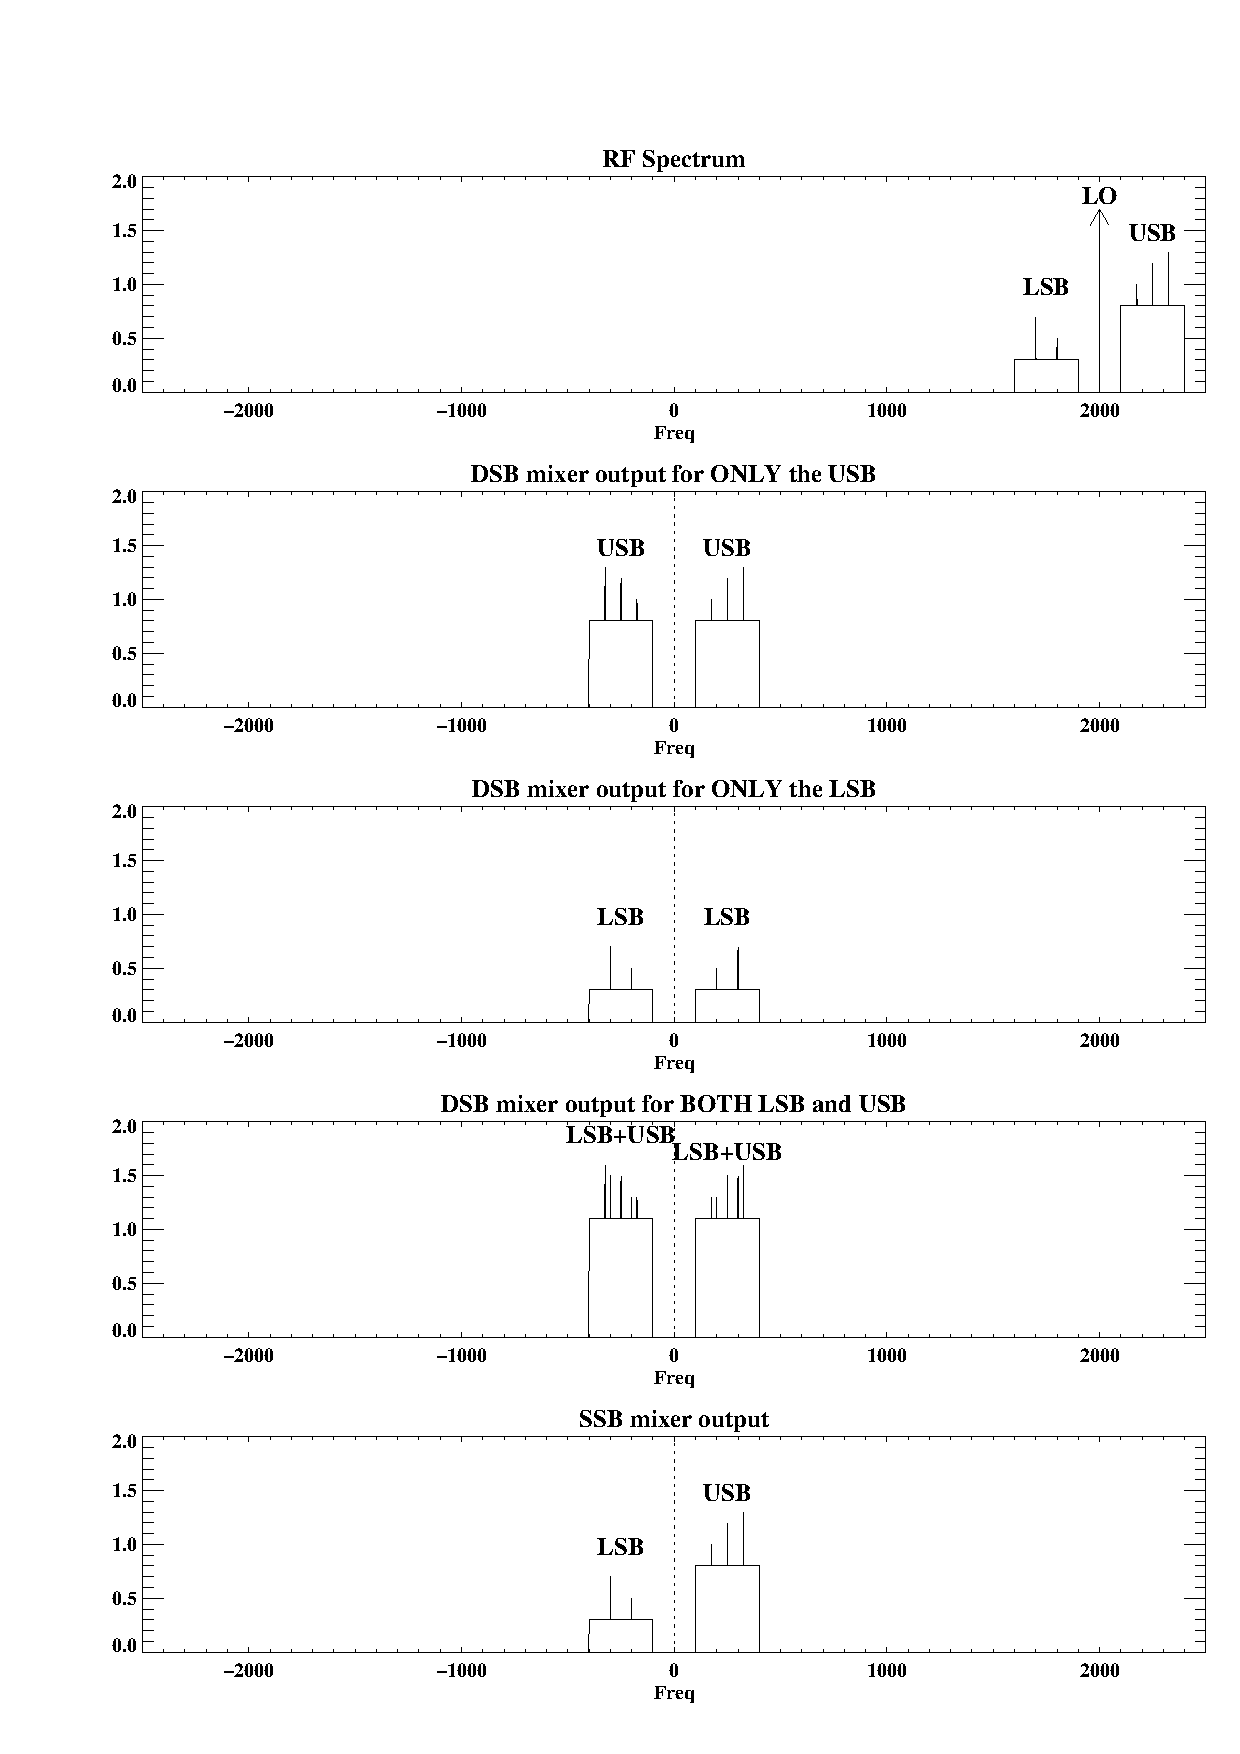
\includegraphics[width=6.5in]{sideband.png}
%\end{center}
%\hspace{-0.5in}
\caption{Upper and lower sidebands in DSB and SSB mixers for a set of
$\delta$-function test signals on top of broad level noise spectra. Top:
  the RF
spectrum. The next two show the USB and LSB {\it individually} when
they undergo the DSB mixing process; panel 4 shows how they both add
together. The bottom panel shows the SSB mixer, which keeps them
separate. \label{sideband}}
\end{figure}
%
        Three things are important here: \begin{enumerate}

        \item {\it The two sidebands---the two different input
frequencies} ($[\omega_{s-}= \omega_0 - \delta \omega]$ and $[\omega_{s+}=
\omega_0 + \delta \omega]$)--- produce the {\it same
symmetric-around-zero pair of IF output frequencies $\pm |\delta
\omega|$}. The DSB mixer
cannot distinguish between the two input frequencies.

        \item Consider how $|\delta \omega|$ depends on $\omega_0$: for
          the upper sideband, ${d |\delta \omega| \over d\omega_0} = -1$,
          while for the lower $d {|\delta \omega| \over d\omega_0} =
          +1$. We hope that the upper three panels of Figure
          \ref{sideband} elucidate the situation.

        \item A value of $E_s$ for one sideband produces a certain mixer
output {\it power}; the same value of $E_s$ for the other sideband
produces the same power. With regard to power, the sidebands are {\it
indistinguishable}.

\end{enumerate}
%
Figure \ref{sideband} illustrates these results. The top panel shows the
original RF spectrum, which consists of signals above the LO (the USB
signal) and below (the LSB). Suppose you use a bandpass filter to
eliminate the LSB. Then you have only the USB, and the second panel
shows the IF spectrum after DSB mixing: the USB appears at both negative
and positive frequencies and the spectrum is symmetric, meaning that the
negative frequencies give exactly the same result as the positive ones.

Now use a bandpass filter to eliminate the USB, leaving only the LSB;
the third panel shows the resulting IF spectrum.

If you didn't use any bandpass filters, then both the LSB and the USB
would appear in the IF spectrum, as in the fourth panel. Looks
complicated! With a DSB mixer, you can't distinguish between LSB and
USB. The LSB and USB are inextricably
mixed and you get the sum of the power spectra. 
The only way can achieve the rejection of either the LSB or the USB is by
using an appropriate {\it bandpass} filter on the input RF spectrum. 

But, nirvana! The bottom panel shows that SSB (Sideband Separating, or
Single Sideband) mixing retains the sideband separation and identity.

\subsection{More Theory: The SSB Mixer}

The SSB mixer has the capability of distinguishing whether the
difference frequency $|\delta f|$ is positive or negative---that
is, it distinguishes between the two sidebands.  The sidebands can, and
usually do, contain completely independent signals; a common example in
everyday life is stereo FM.

Figure\ \ref{ssb} shows a block diagram of the SSB mixer.  The RF input
and the LO are each split by a power splitter so that we have two
identical mixers, one on the left and one on the right, whose outputs
are labelled {\bf Re(IF)} and {\bf Im(IF)}, respectively. The one on
the left is identical to the DSB mixer in figure \ref{dsb}. The one on
the right differs in only one way, which is crucial: its LO is delayed
by $90^\circ$ relative to that on the left. With this, the {\bf Im(IF)}
output lags the {\bf Re(IF)} one by $90^\circ$ in phase. This allows us
to remove the degeneracy in the sidebands by using both inputs to the
Fourier transform, regarding the FT input as complex.

To understand how this works, let's repeat exactly the same math in
equations \ref{eqn4} and \ref{eqn5}, with the addition of a $90^\circ$
phase delay to the l.o.\ signal. In equation \ref{eqn4}, we represented
the LHS l.o.\ by a cosine and used the trig identity `cos times cos = cos +
cos'. With the $90^\circ$ phase delay, the RHS l.o.\ cosine becomes a sine,
and the corresponding trig identity becomes `sin times cos = sin +
sin'. The RHS equivalent of equation \ref{eqn5} becomes
%
\begin{equation}
MO_{\pm, RHS} = {E_s \over 2} \sin [\pm|\delta \omega | t] = \pm {E_s \over
  2}
   \sin [|\delta \omega | t] \ ,
\end{equation}
%
which is identical except that the cosines are sines.

Suppose that the RF input signal a cosine wave in the {\it lower}
sideband, with frequency {\it below} the l.o.\ frequency, i.e.\ $\delta
\omega$ is negative.  Then the LHS
and RHS outputs are sinusoidal, with the two mixer outputs $\propto \cos
[|\delta \omega| t]$ and $-\sin [|\delta \omega| t]$ for the LHS and
RHS, respectively.  These are shown in right panel of Figure
\ref{mixerout}, with the LHS side [$MO_{-,LHS}$] dashed and the RHS side
    [$MO_{-,RHS}$] solid. The two signals are shifted in phase: for the
    RF input being in the {\it lower} sideband, the dashed curve $MO_{-,
      LHS}$ {\it leads} the solid one $MO_{-, RHS}$. When FT'd, this
    corresponds to a {\it negative} IF frequency.

If the RF input signal is a cosine wave in the {\it upper} sideband, with
frequency {\it above} the l.o.\ frequency, $\delta \omega$ is positive
and the situation is
reversed: the dashed curve $MO_{+, LHS}$ {\it lags} the solid
one $MO_{+, RHS}$. When FT'd, this corresponds to a {\it positive}
IF frequency.

\begin{figure}[h]
%        \begin{center}
%\hspace{-0.5in}
%        \leavevmode
        \includegraphics[width=6.5in]{ssbm.png}
%        \end{center}
\caption{Outputs of the first mixers for the two sideband cases. Dashed
  curve shows the {\it left-hand} mixer, solid is the {\it right-hand}
  mixer. Left panel shows $\delta \omega > 0$ ({\it upper}
  sideband---USB); right panel shows $\delta \omega < 0$ ({\it lower}
  sideband---LSB).
\label{mixerout}}
\end{figure}

\section{ON PAPER: YOUR LAB REPORT (Third Week)} \label{report}

\subsection{Handouts}

\begin{enumerate}
\item What should your lab report look like? {\tt
  labreport\_comments.pdf} {\it ``SUGGESTIONS FOR LAB REPORTS''}

\item You must use Latex for your lab report! {\tt sample.pdf} ``LaTex
  Is Your Friend OR ENEMY?????????'' Answer to this question is a
  resounding YES for `Friend'---if you have followed his handout. Use
  LaTex for preparing your lab report!

\item Now's the time for another look at efficient use of the EMACS
  editor, because if you learn the keystoke commands you'll be much
  quicker and save lots of time further down the road: {\tt
    emacs-beg.pdf} {\it ``A Beginners Guide to Emacs''} and the related
  {\tt emacskeyops.pdf} ``Common Editing Tasks and Their EMACS Keystroke
  Counterparts''. Emacs is excellent for everything, including editing
  computer code. Efficient editing means using the keyboard
  instead of the mouse; the second handout gives keystroke commands for
  the most commonly needed editing sequences.

\item You'll need to show plots into your lab report. To do this you
  make PostScript files of your plots. See {\tt bpidl.pdf} {\it ``BPPython---BASIC PLOTTING IN
  Python: PLOTS, MULTIPLE PLOTS, COLORS, MAKING POSTSCRIPT FILES''} Section 6.0.1.

\end{enumerate}
\end{document}
